\documentclass[conference]{IEEEtran}

\usepackage[dvips]{graphicx}
\usepackage{amsmath,amssymb}
\usepackage{algorithm}
\usepackage{algorithmic}
\usepackage{flushend}

\begin{document}
\title{IMSI-based Routing and IMSI Privacy in 5G}
\date{}%date stay empty

\author{
\IEEEauthorblockN{Mohsin Khan, Valtteri Niemi}
\IEEEauthorblockA{University of Helsinki \\ Helsinki Institute of Information and Technology \\ Helsinki, Finland \\ {mohsin.khan, valtteri.niemi}@helsinki.fi\\}
\and
\IEEEauthorblockN{Philip Ginzboorg}
\IEEEauthorblockA{Huawei Technologies \\ Aalto University \\ Finland \\ philip.ginzboorg@huawei.com\\}}
\maketitle

\begin{abstract}
In 5G, identity privacy of a user is proposed to be protected by concealing the identifier of the user. In order to route the concealed identifier to the appropriate destination, certain information of about the international mobile subscriber identity (IMSI) - country code and network code need to be revealed. But, as was recently pointed out, the routing of requests for authentication information between visited and home network and also within the home network, needs more information about the IMSI to be revealed. In this new context, we re-examine published alternative solutions of identity privacy. We find the previously promising solutions e.g., solution based on public key of home network become less promising. We find the solution based on identity based encryption becomes more promising than it was before.
\end{abstract}

\section{Introduction} \label{intro}
One major problem in the realm of identity privacy in mobile networks is to protect the privacy of the international mobile subscriber identity (IMSI). Serious effort has been put to solve this problem in the 3GPP community. Most of the solutions are based on some cryptographic techniques. Comparative analysis between the solutions have been published. There are pros and cons in every solution. 3GPP community is now at the verge of finalizing the specification for the first phase of 5G technology. Identity privacy is a major requirement in 5G. A solution based on public key cryptography is most likely going to be adopted to protect the privacy of IMSI. In this solution, the home network (HN) owns the private key. We call this solution as root-key based solution. The issue of routing requests for authentication information, which has surfaced recently, reduces the effectiveness of this solution. The issue of routing requests for authentication information, which has surfaced recently \cite{SUCIRouting}, reduces the effectiveness of the root-key based solution. Another issue around lawful interception (LI) has been noticed only recently \cite{SUCIRouting}.

In this paper we will do the comparative analysis of the alternative solutions in the light of these two new concerns. We will see that the balance of pros and cons between different solutions change significantly. The root-key based solution which appeared to be quite straightforward and effective solution becomes less effective and requires more implementation effort. On the other hand, a solution based on identity based encryption (IBE) which had its own cons, solves both of the concerns of IMSI-based routing and LI. In this light we will argue that solution based on identity based encryption could the most effective and also fairly straightforward solution to protect the privacy of IMSI.

In order to present a smooth discussion, we need to first explain some background. We will present an abstract view of a mobile network. This view is abstract enough to cover both LTE and 5G, even earlier generations. We will discuss how IMSI is used, how privacy of IMSI is vulnerable. We will also discuss the published solutions to some extent. Then we will explain the new concerns around IMSI-based routing and LI. After that we will explain how the solution based on identity based encryption addresses the two concerns and how the other solutions suffer from them. We will see, these modifications in the analysis make the solution based on identity based encryption the most promising.


\section{Background} \label{background}
\subsubsection{IMSI}
An IMSI is usually presented as a $15$ digit number but can be shorter. The first $3$ digits are the mobile country code (MCC), which are followed by the mobile network code (MNC), either $2$ digits or $3$ digits. The length of the MNC depends on the value of the MCC. The remaining digits are the mobile subscription identification number (MSIN) within the network's customer base \cite{TS23003}. 

Currently, when a user equipment (UE) tries to connect to a network for the first time, the UE has to identify itself using IMSI. Once the UE is identified, an authentication protocol is run in between the UE and the network. If the authentication protocol runs successfully, the network serves the UE with the services the UE is authorized to avail. In all the legacy networks this authentication protocol is a challenge-response based protocol. 


\subsubsection{Mobile Network}
A mobile network consists of UE, serving network (SN) and HN. Both of the SN and HN consist of radio access network (RAN) and core network (CN). The RAN of SN provides the connectivity in between UE and CN of SN. On the other hand, the CN of SN connects itself with the CN of HN via IPX. Note that in a non-roaming situation, the SN and HN are the same network. 

\subsubsection{IMSI Catchers}
There are two more entities which are not part of the network but relevant in our discussion, because they attack the network. They are passive IMSI catchers (PIC) and active IMSI catchers (AIC). The interface UE-SN is a logical interface in between UE and SN. This interface is initially unprotected. The logical interface SN-HN in between SN and HN is protected and the security of this interface is out of the scope of this paper. The PICs eavesdrop on the UE-RAN interface when it is unprotected to extract an IMSI. The AICs impersonate a legitimate SN and run a legitimate-looking protocol with the UE in order to find out the IMSI. HN and UE both know the IMSI and they are trusted. Both PIC and AIC are untrusted. 

\begin{figure}
\begin{center}
% Use the relevant command to insert your figure file.
% For example, with the graphicx package use
  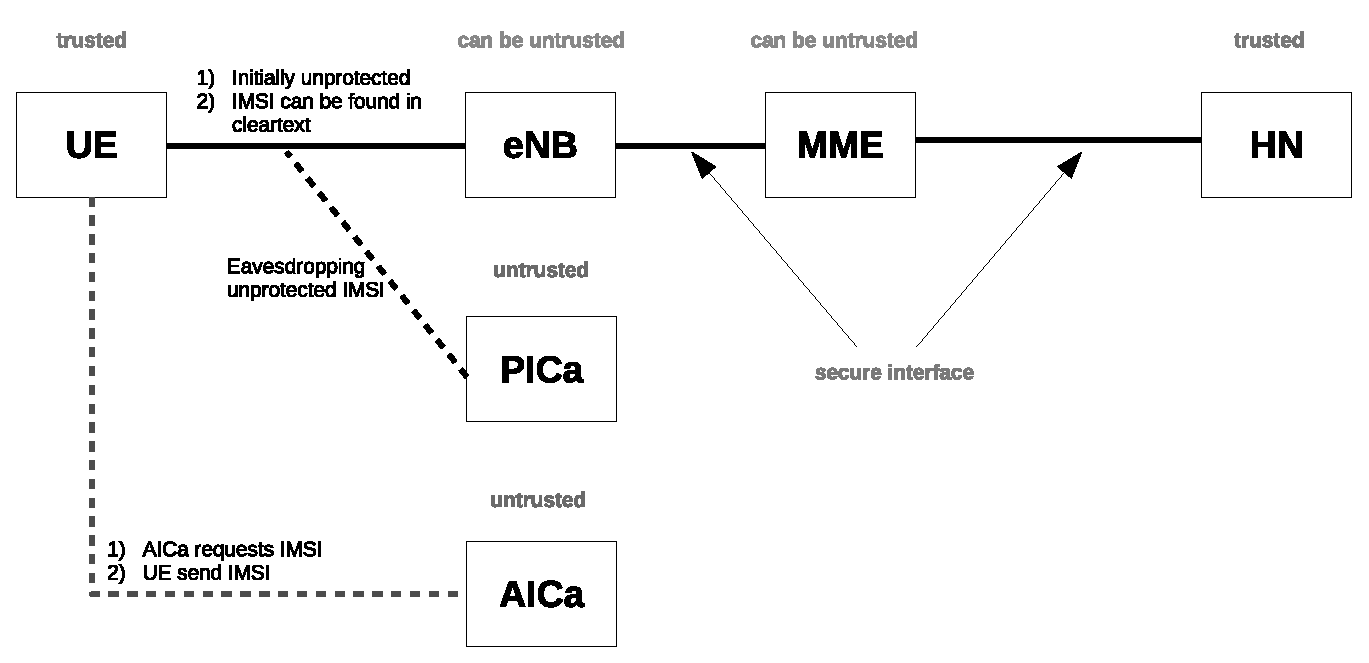
\includegraphics[width=.45\textwidth]{security_architecture_abstraction.eps}
% figure caption is below the figure
\caption{High-level security architecture}
\label{fig:security_architecture_abstraction}       % Give a unique label
\end{center}
\end{figure}


\subsubsection{Solutions Against IMSI catchers}
In legacy networks, the approach of protecting IMSI privacy is to use a temporary identifier instead of the actual IMSI and keep changing the temporary identifier at a feasible frequency. Note that the temporary identifier has to be assigned over a confidentiality protected channel and different entities of the network may assign different temporary identifiers to the UE. In the LTE network, the temporary identifier assigned by serving network (SN) is called globally unique temporary identity (GUTI) and the home network (HN) does not assign any temporary identifier to the UE. However, during the initial attachment of a UE to the SN, the UE has neither a GUTI nor a security context with the SN that can assign it with a GUTI. Besides, GUTI can be lost by either one or both of the UE and the SN. This would force the UE to reveal its IMSI to the SN to keep itself from permanently locked out of the network. This problem gives an opportunity to an active IMSI catcher (AIC) who impersonates a legitimate SN and forces the UE to run the initial attachment protocol. This also gives an opportunity to a passive IMSI catcher (PIC) to eavesdrop the IMSI sent in clear text. To fight against these AICs in 5G, different solutions \cite{pseudonym_valtteri_philip, pseudonym_ericsson, ICTJournal} have been proposed.

\section{Categories of Solutions}
We focus on the solutions using cryptographic techniques. So, we look into the different categories of encryption and see their pros and cons. Modern-day encryption can be broadly categorized into two categories depending on how the keys are used to encrypt and decrypt the message. In symmetric-key encryption the sender and receiver share a secret key which is used for both encryption and decryption. In public-key encryption the receiver has a pair of keys. One of the keys is public and the other is private. The public key is used by the sender to encrypt the message and the private key is used by the receiver to decrypt the message. While the challenge in symmetric key encryption is to create a key known only by the sender and receiver but no one else, one major challenge in public-key encryption is to authenticate the public key.
\begin{figure*}
\begin{center}
% Use the relevant command to insert your figure file.
% For example, with the graphicx package use
  \includegraphics[width=.98\textwidth]{ibc_in_jargon_of_crypto.eps}
% figure caption is below the figure
\caption{IBE in the Taxonomy of Encryption}
\label{fig:ibe_in_the_jargon_of_cryptography}       % Give a unique label
\end{center}
\end{figure*}

Public-key encryption can be further categorized into three more subcategories based on the authentication mechanism used to verify the public keys:
\begin{enumerate}
\item Certificate based encryption
\item Root-key based encryption
\item Identity based encryption
\end{enumerate} 
Figure \ref{fig:ibe_in_the_jargon_of_cryptography} shows this categorization with advantages and disadvantages of the respective categories. Please note that this classification is drawn considering only the encryption operation. Different classifications could be drawn based on other cryptographic operations, e.g., digital signature, hashing or message authentication codes (MAC). Nonetheless, we use this classification, because encryption is the most relevant cryptographic operation for identity confidentiality. 


Next we take a closer look of each category of solution and refer to at least one solution of that category.

\begin{itemize}
\item The pseudonym based solutions as proposed in \cite{pseudonym_ericsson,pseudonym_valtteri_philip,CCS15,SSR15} fall in the category of symmetric key encryption.  In this kind of solutions, temporary identifiers called pseudonyms are assigned to a UE. Next time when the UE tries to identify itself to an SN, it uses a pseudonym instead of IMSI. Periodically, whenever there is an opportunity, the HN sends a new pseudonym to the UE with confidentiality and integrity protection using a symmetric key - that is why it falls under the category of symmetric key encryption.. One such opportunity could be when the HN sends the authentication vector to an SN.

\item In the certificate based encryption, the public key is signed by a trusted third party. The sender has to be pre-provisioned with the root certificate so that the sender can authenticate the public key of the receiver. Use of certificate based public-key encryption to conceal long-term identity has been suggested in 3GPP TR 33.821 \cite{TR33821}. To use certificate based public-key cryptography, we need to figure out who are the root certificate authorities (CA) and who else can be a CA, who owns a public key, how a certificate can be revoked, and how the UE can be re-provisioned with a new root certificate if needed. Different solutions can be devised based on the choice of root CAs and other CAs. 


One variant uses a global root of trust. There is a global entity trusted by everyone. Using this trusted global entity, a chain of trust can be established. The SN presents the certificate to a UE trying to attach. The UE verifies the certificate. If the verification result is positive, the UE encrypts its IMSI using the public key of the SN and sends to the SN. 

In another variant, the HN of a subscriber is the root CA. The HN generates a public-private key pair and generates a certificate of the public key signed by the HN itself. A UE is provisioned with this self signed certificate. An SN interested to serve a UE also generates a public-private key pair. The SN obtains a certificate for its public key from the HN. The UE sends its MCC and MNC to the SN. The SN looks up for the relevant certificate. In case it exists at the disposal of the SN, the SN sends it to the UE. The UE verifies the certificate. If the certificate is verified as valid, then the UE sends the IMSI to the SN encrypted by the public key of the SN.

There is also a variant where there are no other CA than the root CA. Hence the chain of certificates is very short. Only an HN can be a CA. The certificates of all the SNs a UE might visit are pre-provisioned to the UE by the HN. When a UE attempts to attach to an SN, the UE encrypts the IMSI with the public key of the SN which is already provisioned to the UE. If the public key of an SN is revoked, the HN has to provision the revocation to the UE.

\item In the root-key based encryption, no runtime authentication of the public key is required, because a very limited number of public keys are used in the system and all the senders are pre-provisioned with all the existing public keys. Use of root-key has been proposed in 3GPP TR 33.899 in solution \#7.3. In this approach only one pair of public-private key pair exists. This key pair is owned by the HN and we call it to be the root-key. The HN provisions the public key to all its UEs.  Instead of sending the IMSI, the UE encrypts the IMSI with the public root key and sends the result to the SN along with MCC and MNC. The SN sends the encrypted IMSI to the HN. The HN decrypts the IMSI and sends the IMSI back to the SN along with an authentication vector (AV).

\item In IBE, the public key of a receiver is computed from the identity of the receiver and the public key of a trusted third party known as private key generator (PKG). The public key of the trusted third party has to be provisioned to the sender. The private key of the receiver is computed as a function of the identity of the receiver and the private key of the PKG. The private key of the receiver has to be provisioned to the receiver by the PKG. In IBE based solution, the HN is the PKG. The HN has a public-private key pair. The UEs are provisioned with the public key of the HN. The SNs which have a roaming agreements with the HN are also provisioned with their respective private keys by the HN. When a UE identifies itself with IMSI, it encrypts the IMSI using the public key of the SN. The UE computes the public key of the SN as function of the identity of the SN and the public key of the HN. The most interesting aspect of this solution is that there is no certificate involved and the SN can decrypt the encrypted IMSI.
\end{itemize}

\section{IMSI-based Routing and LI}
The interworking between mobile network operators happens via IP Exchange (IPX). Initially, when a user identifies itself with IMSI, this identifier needs to be routed to the appropriate HN entity that stores the authentication related information, e.g., secret key. In an ideal situation, the MCC and MNC should be enough to route an IMSI to the relevant entity in the HN. However, there are situations when MCC and MNC are not enough. 

There is a concept called mobile virtual network operator (MVNO). An MVNO purchases services in bulk from an MNO and retails out to its own customers. An MVNO's has its own subscription server. Consequently, an IMSI needs to be routed to the MVNO's subscription server. However, all the subscribers of the MVNO would share the same MCC and MNC as the MNO that it bought the service from. So, MCC and MNC are not enough information to route an IMSI to an MVNO. The IPX needs to know more information from the MSIN - the last part of the IMSI.

There is another concept called unified data management (UDM). The whole subscriber base of an MNO may be split in multiples instances of a UDM. So, while routing the IMSI to an MNO, it needs to be routed to the UDM in which the IMSI belongs to. In this case too, the routing to appropriate UDM requires more information from the MSIN.

If the MSIN is concealed by the UE, and the subscriber belongs to an MVNO, then the IPX can not route it to the appropriate MVNO. If the subscriber belongs to a particular UDM of an MNO, IPX can route it to the MNO. However, before it can be routed to the appropriate UDM, the MSIN needs to be decrypted. Decrypting the MSIN before routing it to the UDM undermines, at least partially, the purpose of UDM.

In this light, it appears that some information of the MSIN must not be concealed or some routing information has to accompany the concealed MSIN to enable the correct routing. In either way, this extra information reveals information about the user and the probability of the user being identified goes higher. If information equivalent to $n$ digits of MSIN is revealed, the probability of identifying a user goes up by a factor of $10^n$ - for $n=4$, it becomes ten thousand times bigger. Nonetheless, notice that the solutions in which the MSIN is decrypted at SN e.g., IBE based solution do not suffer this weakened privacy.

There is another concern regarding LI. According to specification, the SNs should be able to identify a user with the permanent identity - IMSI. However, if the MSIN is concealed and the SN can not reveal the MSIN then the SN has to learn the MSIN from the HN. The concern is about how the SN can trust that the HN is telling the truth. Solutions have been proposed in the 3GPP community to solve this problem. However, the proposed solution adds some overhead in the authentication process. Again notice that the solutions in which MSIN can be decrypted in the SN do not have this problem. The SN would learn the MSIN from the UE. So, if the authentication becomes successful, the SN can trust that the user is the one who the user claims to be, unless the HN and the user collude to fool the SN.

\section{Qualitative Comparison of Different Categories of Solutions}
Qualitative comparison of different solutions based on different criteria was presented in \cite{ICTJournal}. In this paper we take the same approach. We choose those criteria which we believe makes a difference between solutions. However, we only compare according to the solution categories.  We have discussed two different categories of solutions: pseudonym based and public-key based. We have categorized the different public-key technologies into three categories: certificate based, root-key based and identity based. In Table \ref{table:comparison}, we present a comparison among the different solutions based on different criteria. We indicate the performance of the solutions according to different criteria according the following symbols

\begin{itemize}
\item + is good 
\item - is not good
\item +- is somewhat okay
\item ++ is very good
\end{itemize}

\subsection{Immunity Against AIC} This is the most important criterion because the whole effort is to defeat the AICs. An AIC can still learn the MCC and MNC in pseudonym based and root-key based solutions. Because of the concerns around IMSI-based routing, pseudonym based and root-key solutions have to reveal more information from MSIN. It makes them less immune against AIC. So, we evaluate them with +-. The certificate based solution with global PKI can conceal even MCC and MNC. So, we evaluate them with ++. In IBE based solution, only MCC and MNC needs to be revealed. So we evaluate it with +.

\subsection{LI} Both the pseudonym based and root-key based solution requires extra overhead in the identification process. So we evaluate them with +-. Both certificate based and IBE based solution works quite well to facilitate LI because the SN gets the IMSI directly from the UE. So, we evaluate them with +.

\subsection{Deployment and Maintenance Effort}
Pseudonym based approach is relatively easy to deploy but makes the subscription database very sensitive to any changes, hence the maintenance becomes difficult. So, we rate this with +-. Certificate based solutions require setting up PKI and maintaining it. That is a lot of effort. So we rate certificate based solution with -. Root-key based and IBE based solutions are fairly easy to deploy and maintain. So we rate them with +.

\subsection{Transparency to the Legacy SNs}
Pseudonym based solution would be transparent to the legacy SNs if the trust issue around LI was not there. To provide the trust, the SN would need change. Consequently, even though previously it was a very important advantage of pseudonym based approach, it becomes a disadvantage now. So we rate this with -. However, no other solutions are transparent to SNs. So we rate all of them with -.

\subsection{Signalling overhead}
In pseudonym based solution, no extra signalling overhead is added on top of what exists in the legacy networks. So we rate it with ++.
Certificate based solutions require an extra round trip between the UE and SN to exchange and verify the certificate. In one variant of a certificate based solution, this extra round trip could be removed at the expense of provisioning the certificate of an SN to a UE before the UE goes roaming to the SN. All the certificate based solutions have the requirement of exchanging certificates and verifying them. This creates signalling which consequently affect the latency. So we rate certificate based solution with -. The root-key and IBE based solutions do not require any extra round trips or certificates, hence they have less signalling overhead compared to certificate based solutions. So we rate them with +.

\subsection{Computational overhead}
Pseudonym based solutions require some extra computation in the HN to generate next pseudonym of a user randomly. However, this is less complex in comparison with public key encryption. So, we rate it with ++. Certificate based solutions require to exchange and verify the certificate and compute public key encryption/decryption. This creates computational overhead. So, we rate it with -. However, both root-key and IBE based solutions require public key encryption and decryption but do not require verifying certificates. So we rate them with +.

\subsection{Latency}
In pseudonym based solution, no extra signalling overhead, extra round trip or longer message length is introduced on top of what exists in the legacy networks. Consequently the latency is not affected much. So we rate it with +. Certificate based solutions require an extra round trip between the UE and SN to exchange and verify the certificates, computes public key encryption and have longer message length. All these affect the latency. So we rate certificate based solution with -. The root-key and IBE based solutions do not require any extra round trips or certificates. However, they compute public key encryption and have longer message length. Hence the latency is affected. So we rate them with +-.


\subsection{Key revocation}
Pseudonym based solution is a symmetric-key based solution. So it does not require any key revocation. So, we rate it with ++. However, all the public key based solutions require a mechanism of key revocation. In certificate based solution, to access the revocation list, a user has to connect to an SN. On the other hand, in IBE based solutions, revocation is inherently complicated. One solution around this is to use short expiry time for the public keys of the SNs. By doing so, key revocation increases some overhead. So we rate both of them with -. In root key based solution no revocation is required because there is only one public key. So we rate it with +.

\subsection{Maturity}
We also look at the solutions from the point of view of the maturity of the technology. Use of pseudonyms for privacy purpose is not yet a very matured technology. Use of IBE is not yet widespread. So we rate both of them with -. However, certificate based public-key encryption technology is widespread and matured. Use of root-key can be viewed as a special case of certificate based public-key. So, we rate both of certificate based and root-key based solutions with +.

\subsection{Mutual authentication} It is possible that in future there might be a need of mutual authentication between the UE and the SN without the intervention of the HN. In this respect we notice that pseudonym based and root-key based solution can not be used for mutual authentication. This is because, in these cases the IMSI is not visible to the SN without consulting with the HN. So, we rate these two categories with -. However, Certificate based and IBE based solutions can be extended into a mutual authentication protocol between UE and SN. One example can be found in \cite{ICTJournal}. So, we rate both of these two categories with +.
   

\subsection{Summary of the Comparison}
Looking at the table, it seems evident that IBE based solution is the most promising solution. Certificate based approach is good in preventing AIC and handling the requirement of lawful interception. But the solution is costly in almost all other aspects. So maybe, the industry is not yet ready to spend such expenses to provide user identity privacy. Even though pseudonym based approach is inexpensive from almost all the aspects, it becomes a bit less effective to achieve its original purpose - immunity against AIC. Because of the LI issues, it also loses its most important merit - transparency with legacy SNs. The root-key based approach is also a bit less effective in serving its original purpose - immunity against AIC. It also makes the lawful interception a bit more complicated than that of IBE based solution. However, key revocation in IBE may have some latency whereas no key revocation is required in root-key. But still, considering the effectiveness of the solution, we would like to conclude that IBE based solution is a better choice than the root-key based solution.


\begin{table*}
\begin{small}
\begin{center}
\caption{Comparative evaluation of the solutions}
\begin{tabular}[t]{|l|c|c|c|c|}
\hline
%\multicolumn{1}{|c|}{} & \multicolumn{1}{|c|}{} & \multicolumn{7}{|c|}{\textbf{Public-key based Solutions}}\\
%\cline{3-9}
\multicolumn{1}{|c|}{\textbf{Criteria}} & \multicolumn{1}{|c|}{\textbf{Pseudonym}} & \multicolumn{1}{|c|}{\textbf{Certificate based}} & \multicolumn{1}{|c|}{\textbf{Root-key}} & \multicolumn{1}{|c|}{\textbf{IBE based}}\\
%\cline{3-5} \cline{7-9}
%\textbf{} &  & \textbf{V1} & \textbf{V2} & \textbf{V3} & \textbf{} & \textbf{JPL} & \textbf{PEMMA} & \textbf{PEFMA}\\
\hline \hline
Immunity to AIC & +- & ++ & +- & + \\ \hline
Lawful interception & +- & + & +- & + \\ \hline
Deployment and Maintenance Effort & +- & - & + & + \\ \hline
Transparency to the Legacy SNs & - & - & - & - \\ \hline
Signalling overhead & + + & - & + & + \\ \hline
Computational overhead & ++ & - & + & + \\ \hline
Latency & + & - & +- & +- \\ \hline
Key revocation & ++ & - & + & - \\ \hline
Maturity  & - & + & + & - \\ \hline
Mutual Authentication & - & + & - & + \\ \hline
\end{tabular}
\label{table:comparison}
\end{center}
\end{small}
\end{table*}


\section{Conclusion}
Recently two concerns were raised in 3GPP community regarding the routing of IMSIs and LI. These two concerns are now affecting the effectiveness of different alternative solutions of identity privacy. We have analysed the impact of these two concerns in different solutions made a qualitative comparison between different categories of solutions. We have surprisingly found that IBE based solution outperforms the root-key based solution. In the 3GPP community root-key based solution is most likely going to be standardised. Nonetheless, based on this analysis, it would be worth for 3GPP community to reconsider their decision.

\section*{Acknowledgment}


\begin{thebibliography}{6}

\bibitem{NGMN_white_paper} NGMN 5G White Paper V1.0 [cited Jan, 2017]. Available at: https://www.ngmn.org/uploads/media/\\NGMN\_5G\_White\_Paper\_V1\_0.pdf

\bibitem{TR33899} 3GPP TR 33.899 V0.6.0 [cited Jan, 2017]. Available at: https://portal.3gpp.org/desktopmodules/Specifications/\\SpecificationDetails.aspx?specificationId=3045

\bibitem{TS23003} 3GPP TS 23.003 V14.2.0 [cited Jan, 2017]. Available at: https://portal.3gpp.org/desktopmodules/Specifications/\\SpecificationDetails.aspx?specificationId=729

\bibitem{TR21905} 3GPP TR 21.905 [cited Jan, 2017]. Available at: https://portal.3gpp.org/desktopmodules/Specifications/\\SpecificationDetails.aspx?specificationId=558


\bibitem{pseudonym_ericsson} Karl Norrman, Mats N\"aslund, Elena Dubrova: Protecting IMSI and User Privacy in 5G Networks. 2nd International Workshop on 5G Security

\bibitem{pseudonym_valtteri_philip} Philip Ginzboorg,  Valtteri Niemi: Privacy of the long-term identities in cellular networks. Proceedings of the 9th EAI International Conference on Mobile Multimedia Communications, Pages 167-175

\bibitem{CCS15} Fabian van~den Broek, Roel Verdult, Joeri de~Ruiter: Defeating IMSI Catchers. Proceedings of the 22Nd ACM SIGSAC Conference on Computer and Communications Security, CCS '15, pages 340--351. ACM, 2015.


\bibitem{SSR15} Mohammed Shafiul~Alam Khan and Chris~J. Mitchell Improving Air Interface User Privacy in Mobile Telephony. In Second International Conference, SSR 2015, Proceedings, pages 165--184. Springer International Publishing, 2015.


\bibitem{TR33821} 3GPP. 3GPP TR 33.821 Available at https://portal.3gpp.org/desktopmodules/Specifications/\\SpecificationDetails.aspx?specificationId=2311, 2009.

\bibitem{ICTJournal} Mohsin Khan, Valtteri Niemi: Privacy Enhanced Fast Mutual Authentication in 5G Network Using
Identity Based Encryption. In Journal of ICT Standardization, Vol 5, Issue 1

\bibitem{SUCIRouting} 3GPP TSG SA WG3 (Security) Meeting \#90-Bis: S3-180723, Requirement on routing SUCI. Available at
ftp://ftp.3gpp.org/TSG\_SA/WG3\_Security/TSGS3\_90Bis\_SanDiego/Docs/

\bibitem{Li Requirement} 3GPP TSG SA WG3 (Security) Meeting \#90-Bis: S3-180590,Requirement for SUPI privacy and LI. Available at 
ftp://ftp.3gpp.org/TSG\_SA/WG3\_Security/TSGS3\_90Bis\_SanDiego/Docs/

%\bibitem{Cover}
%\textit{(Example for books)} T.M.Cover and J.A. Thomas, \emph{Elements of Information Theory}. New York: Wiley, 1991.

%\bibitem{Dobrushin}
%\textit{(Example for articles)} R.L. Dobrushin, ``Optimum information transmission through a channel with unknown parameters'',  \emph{Radiotech.Electron.}, vol.4, Dec.1959, pp. 1951-1956.

%\bibitem{Blachman}
%\textit{(Example for articles)} N.M. Blachman, ``Communication as a game'', \emph{in Proc. WESCON Conf.}, Aug. 1957, pp. 61-66.

%\bibitem{IEEE}
%\textit{(Example for web-links)} IEEE official website, Manuscript Templates for Conference Proceedings, Web: http://www.ieee.org/conferences\_events/conferences/publishing/templates.\newline html.

%\bibitem{Elissa}
%\textit{(Example for unpublished references)} K. Elissa, ``Title of paper if known'', unpublished.

%\bibitem{Nicole}
%\textit{(Example for references have been accepted for publication)} R. Nicole, ``Title of paper with only first word capitalized'', J. Name Stand. Abbrev., in press.

\end{thebibliography}

\end{document}